\section{Descrizione dell'architettura}
\subsection{Architettura frontend}
\subsubsection{Design pattern architetturale}

\paragraph{Redux-Toolkit}
I componenti che costituiscono l'architettura frontend utilizzata seguono il
pattern offerto dalla libreria Redux-Toolkit. Redux-Toolkit è pensato per
integrarsi con React e il principale vantaggio che offre è quello di poter
gestire i dati condivisi tra i componenti React in modo centralizzato
semplificando la gestione dello stato globale dell'applicazione. Inoltre
Redux-Toolkit è un wrapper che semplifica l'utilizzo di Redux in modo tale da
scrivere meno codice e commettere meno errori durante lo sviluppo.

I componenti che formano l'architettura di Redux-Toolkit sono:
\begin{itemize}
      \item \textbf{Store:} componente che contiene lo stato globale dell'applicazione.
            All'avvio dell'applicazione viene configurato utilizzando RootReducer e i componenti che utilizzano
            lo stato globale si mettono in ascolto dello store in modo da venire renderizzati ogni volta che un dato
            di interesse cambia valore. Questo modo di operare può essere visto come un pattern Observer in
            cui lo store è il Subject e gli Observer sono i componenti React che osservano i cambiamenti dello store;
      \item \textbf{RootReducer:} componente utilizzato per configurare lo store combinando le slice;
      \item \textbf{Slice:} componente che contiene un proprio stato che rappresenta una porzione dello stato globale
            dell'applicazione, i reducer che operano su tale stato e i selector per consentire ai suoi client il
            reperimento dei dati;
      \item \textbf{Reducer:} componente che riceve come parametri uno stato iniziale (InitialState) e un'action
            (composta da un type e un payload) e restituisce lo stato dopo aver operato sui dati.
            Il type rappresenta una stringa univoca che ha lo scopo di identificare la specifica action che si intende eseguire.
            Il payload è un oggetto che contiene i dati necessari per l'esecuzione dell'action.
            React-Toolkit gestisce le chiamate ai reducer in seguito ai dispatch delle action che avvengono
            specificando solamente l'oggetto che rappresenta il payload;
            Con il termine dispatch si intende una funzione che viene chiamata per inviare una action allo store di Redux e innescare un cambiamento dello stato.
      \item \textbf{Action:} oggetto composto da un type e da un payload di cui viene effettuato il dispatch quando
            opportuno.
      \item \textbf{State:} componente che contiene i dati di una slice su cui essa opera.
            Importante sottolineare che Redux-Toolkit garantisce l'immutabilità dei dati in modo che i reducer restituiscano delle copie dello stato in modo che esso non possa venire
            modificato dall'esterno è utilizzato in modo improprio.
            L'unico modo per modificare i dati dello stato globale è quindi con il dispatch di un'action;
      \item \textbf{Selector:} funzione che prende lo stato corrente di una slice come argomento e ritorna un sottoinsieme
            specifico del suo stato. In altre parole, un selector consente di selezionare una parte specifica
            dello stato in modo da poterla utilizzare in modo isolato all'interno di un componente React.
\end{itemize}

%% TODO FLUX
\paragraph{Flux Pattern}
Redux Toolkit, in quanto astrazione della libreria Redux, implementa il pattern architetturale Flux,
il quale assicura un flusso di dati unidirezionale e prevedibile dal modello alla view.
Il pattern Flux è principalmente composto da 3 parti:
\begin{itemize}
      \item \textbf{Dispatcher}: Un hub centrale che riceve le Actions e le distribuisce agli Store.
      \item \textbf{Stores}:  Contengono lo stato dell'applicazione e la logica per aggiornarlo in risposta alle Actions.
      \item \textbf{Views}: Visualizzano i dati provenienti dagli Stores e inviano le Actions in risposta alle interazioni dell'utente.
\end{itemize}
Nel suo funzionamento, Flux condivide alcune similitudini con il pattern MVC puro:
quando l'utente interagisce con la View, questa invia un'action (un segnale descrittivo) tramite un Dispatcher centrale ai vari Stores.
Gli Stores contengono la business logic e, in seguito a una modifica del loro stato, notificano le Views che li utilizzano, innescando un aggiornamento.

Questo pattern quindi offre diversi vantaggi come:
\begin{itemize}
      \item \textbf{Separazione delle responsabilità}: Grazie alla suddivisione in Dispatcher, Stores, Views,
      ogni componente ha un compito specifico. Ciò semplifica la manutenzione e l’estensione del sistema.
      \item \textbf{Testabilità}: La struttura a stores e dispatchers facilita l’esecuzione di test unitari e di integrazione, poichè
      ciascuno store, o nel caso di Redux-Toolkit ciascuno slice può essere testato in isolamento.
      \item \textbf{Flusso di dati unidirezionale}: Essendo unidirezionale facilita la comprensione della propagazione delle modifiche,
       ma semplifica notevolmente anche il debugging, evitando la ricerca di aggiornamenti distribuiti e difficili da localizzare.
      \item \textbf{Gestione dello stato centralizzata}: Gli Stores fungono da contenitori centralizzati per lo stato dell'applicazione. 
      Questo rende più facile condividere lo stato tra diversi componenti senza ricorrere a complesse catene di props o a state globale difficile da gestire.
\end{itemize}


\subsubsection{Elenco dei componenti}
Poiché il team di sviluppo frontend utilizzerà Redux per la gestione dello
stato, l'applicazione sarà strutturata principalmente attraverso la
suddivisione del codice in slice, state e action.
\paragraph{Slice}
Le slice contengono una porzione dello stato globale dell'applicazione che è
gestita da un reducer specifico.
\begin{itemize}
      \item \textbf{DataSlice:} componente che gestisce lo stato e contiene i dati relativi al dataset selezionato dall'utente;
      \item \textbf{AppSlice:} componente che gestisce lo stato dell'applicazione come errori e caricamenti;
      \item \textbf{DataSourceSlice:} componente che gestisce lo stato e contiene l'elenco dei dataset selezionabili dall'utente e il dataset selezionato;
      \item \textbf{FilterOptionSlice:} componente che gestisce lo stato e contiene le opzioni di filtraggio dei valori;
      \item \textbf{ViewOptionSlice:} componente che gestisce lo stato e contiene le opzioni di visibilità del piano medio;
      \item \textbf{RaycastHitSlice:} componente che gestisce lo stato e contiene le informazioni relative al raycasting.
\end{itemize}
\paragraph{State}
Gli state, definiti all'interno di ciascuna slice, si combinano per formare lo
stato globale iniziale, gestito dallo store.
\begin{itemize}
      \item \textbf{DataState:} componente che contiene i dati relativi al dateset selezionato dall'utente;
      \item \textbf{AppState:} componente che contiene i dati relativi allo stato attuale dell'applicazione;
      \item \textbf{DataSourceState:} componente che contiene le informazioni principali di tutti i dataset e quelle relative al dataset selezionato dall'utente;
      \item \textbf{FilterOptionState:} componente che contiene i dati relativi alle opzioni di filtraggio selezionate dall'utente;
      \item \textbf{ViewOptionState:} componente che contiene i dati relativi alle opzioni di visibilità del piano medio all'interno dell'ambiente 3D;
      \item \textbf{RaycastHitState:} componente che contiene i dati relativi al raycast, utilizzati per l'interazione con le barre del grafico 3D.
\end{itemize}
\paragraph{Action}
Le action, emesse dai componenti, vengono inviate ai reducer per aggiornare lo
stato corrispondente. Ogni action è caratterizzata da un type e da un payload,
che viene utilizzato dalle slice per modificare lo stato. Per convenzione il
nome delle action segue il formato: \\
\begin{center}
      \textbf{[nome slice].[nome funzione]}.
\end{center}
\begin{itemize}
      \item \textbf{DataSlice.requestData:} action asincrona emessa per recuperare dal server i dati del dataset selezionato. \\ Payload: nessuno;
      \item \textbf{DataSlice.filterFirstN:} action emessa per filtrare i dati, visualizzando solo i primi N valori più alti o più bassi. \\ Payload: FilterPayload;
      \item \textbf{DataSlice.filterByValue:} action emessa per filtrare i dati, visualizzando solo quelli con un valore maggiore o minore rispetto al valore della barra del grafico selezionata.\\ Payload: FilterPayload;
      \item \textbf{DataSlice.filterByAverage:} action emessa per filtrare i dati, visualizzando solo quelli con un valore maggiore o minore rispetto alla media globale. \\ Payload: boolean $\rightarrow$ maggiore o minore;
      \item \textbf{DataSourceSlice.requestDatasets:} action asincrona emessa per recuperare l'elenco delle informazioni relative a tutti i dataset disponibili. \\ Payload: nessuno;
      \item \textbf{DataSourceSlice.trySetCurrentDataset:} action emessa per determinare se il dataset selezionato dall'utente esiste. \\ Payload: number $\rightarrow$ ID del dataset;
      \item \textbf{DataSourceSlice.setCurrentDataset:} action emessa per aggiornare il dataset selezionato dall'utente. \\ Payload: DatasetInfo$\|$undefined $\rightarrow$ informazioni sul dataset, se esistente;
      \item \textbf{ViewOptionSlice.toggleAveragePlane:} action emessa per aggiornare il flag di visibilità del piano medio globale nell'ambiente 3D. \\ Payload: boolean;
      \item \textbf{FilterOptionSlice.toggleIsGreater:} action emessa per aggiornare il flag che determina se il filtraggio deve essere eseguito per valori maggiori o minori. \\ Payload: boolean;
      \item \textbf{RaycastHitSlice.setHit:} action emessa per aggiornare la barra selezionata nel grafico 3D. \\ Payload: number $\rightarrow$ ID della barra;
      \item \textbf{RaycastHitSlice.setTooltipPosition:} action emessa per aggiornare la posizione del tooltip in base alla posizione del puntatore.\\ Payload: Vector3 $\rightarrow$ posizione del puntatore.
\end{itemize}
\paragraph{Classi}
Classi offerte dalle librerie utilizzate:
\begin{itemize}
      \item \textbf{Provider:} componente Redux che rende lo store accessibile a tutti i componenti dell'applicazione, "avvolgendo" il componente principale App e accettando lo store come prop;
      \item \textbf{Store:} componente Redux che traccia lo stato dell'applicazione, contiene il reducer principale per la gestione delle action e fornisce metodi per accedere allo stato,
            registra i listener per le modifiche di stato;
      \item \textbf{RootReducer:} componente Redux che combina tutti i reducer dell'applicazione in uno stato
            globale. Questa funzione viene passata allo store per gestire lo stato complessivo dell'applicazione;
      \item \textbf{FontLoader:} classe utility di Three.js che permette di caricare dati di font in formato JSON per poi generare mesh di testo in ambienti tridimensionali;
      \item \textbf{GSAP:} classe utility della libreria GSAP che permette di creare animazioni sia dell'interfaccia utente (UI) e sia all'interno dell'ambiente 3D con facilità e poco codice.
      \item \textbf{Canvas:} componente React Three Fiber che comprende gli elementi grafici che vanno a costituire la scena 3D.
            Fornisce una telecamera e una scena con una serie di prop opzionali utili alla configurazione dell'ambiente 3D;
      \item \textbf{OrbitControls:} componente React Three Drei che abilita la navigazione e la manipolazione della telecamera utilizzando gli input del mouse;
      \item \textbf{AmbientLight:} componente React Three Fiber che fornisce un'illuminazione uniforme senza ombre alla scena 3D;
      \item \textbf{PointLight:} componente React Three Fiber che fornisce un'illuminazione emessa da un punto verso tutte le direzioni nella scena 3D;
\end{itemize}
Classi definite dal team:
\begin{itemize}
      \item \textbf{Dataset:} classe che rappresenta l'intero dataset con relative etichette e legenda;
      \item \textbf{Legend:} classe che rappresenta la legenda di un dataset;
      \item \textbf{Data:} classe che rappresenta un singolo dato, visualizzato come una barra nel grafico;
      \item \textbf{AppState:} classe che rappresenta lo stato dell'applicazione;
      \item \textbf{DatasetInfo:} classe che rappresenta un dataset e ne memorizza le informazioni principali;
      \item \textbf{RaycastHit:} classe che rappresenta il punto di intersezione tra il puntatore e una barra del grafico;
      \item \textbf{FilterPayload:} classe che rappresenta il payload da inviare alle action di filtraggio del DataSlice;
      \item \textbf{CustomError:} classe astratta che rappresenta un errore generico;
      \item \textbf{TooManyRequestsError:} classe che rappresenta un errore di superamento del limite massimo di richieste effettuate;
      \item \textbf{NotFoundError:} classe che rappresenta un errore dovuto alla richiesta di dati non trovati;
      \item \textbf{ServerError:} classe che rappresenta un errore interno al server.
\end{itemize}
\paragraph{Componenti React UI}
I seguenti componenti, sviluppati dal team, visualizzano i dati dello stato che
compongono la UI:
\begin{itemize}
      \item \textbf{ErrorPage:} componente che visualizza la pagina di errore dell'applicazione;
      \item \textbf{HomePage:} componente che visualizza la homepage dell'applicazione;
      \item \textbf{DatasetItem:} componente che visualizza le informazioni relative a un dataset.
      \item \textbf{UI:} componente che aggrega i componenti grafici che compongono la UI;
            \begin{itemize}
                  \item \textbf{Options:} componente che aggrega le opzioni generali;
                  \item \textbf{FilterOptions:} componente che aggrega le opzioni di filtraggio;
                  \item \textbf{Tooltip:} componente che visualizza un tooltip con i dettagli di una barra;
            \end{itemize}
      \item \textbf{DataTable:} componente che visualizza una tabella contenente tutti i valori del dataset selezionato;
      \item \textbf{FilterModOption:} componente per la configurazione del tipo di filtraggio dati;
      \item \textbf{AveragePlaneOption:} componente per la selezione della visibilità del piano medio;
      \item \textbf{NFilter:} componente che consente l'inserimento di un valore N e applica il filtraggio ai primi N valori più alti o più bassi;
      \item \textbf{Filter:} componente che implementa un filtro generico capace di filtrare valori superiori o inferiori rispetto a un dato valore di riferimento;
\end{itemize}
\paragraph{Componenti tridimensionali di Three.js}
I seguenti componenti visualizzano i dati del dataset all'interno dell'ambiente
3D tramite un grafico.
\begin{itemize}
      \item \textbf{EnvironmentPage:} componente che permette di visualizzare la pagina in cui viene renderizzato l'ambiente 3D;
      \item \textbf{CustomCanvas:} componente che fornisce una telecamera e una scena tridimensionale, configurabili tramite prop opzionali;
      \item \textbf{BarChart:} componente che permette di visualizzare un grafico 3D;
      \item \textbf{AveragePlane:} componente che permette di visualizzare il piano medio globale;
      \item \textbf{Bars:} componente che permette di visualizzare le barre di un grafico 3D;
      \item \textbf{Raycaster:} componente che gestisce la logica di intersezione tra il puntatore e le barre del grafico;
      \item \textbf{ZAxis:} componente che rappresenta l'asse Z del grafico 3D;
      \item \textbf{XAxis:} componente che rappresenta l'asse X del grafico 3D;
      \item \textbf{YAxis:} componente che rappresenta l'asse Y del grafico 3D;
      \item \textbf{Lights:} componente che gestisce l'illuminazione all'interno della scena tridimensionale.
\end{itemize}

\pagebreak

\subsubsection{Architettura logica}
I diagrammi delle classi sono organizzati per slice e componenti React per una
lettura più semplice. Sono presenti anche diagrammi che mostrano le dipendenze
generali tra i componenti React.\\\\ \textbf{Nota:}\\ I rettangoli che
rappresentano le classi sono colorati per distinguere i diversi tipi di
componenti.
\begin{itemize}
      \item \textbf{Bianco:} normali classi;
      \item \textbf{Giallo:} action Redux;
      \item \textbf{Blu:} componenti React;
      \item \textbf{Verde:} componenti React della libreria React Three Fiber.
\end{itemize}

\paragraph{DataSlice}
\begin{figure}[h!] \centering
      \includegraphics[scale=0.3]{template/images/uml_front/logic/DataSlice.png}
      \caption{DataSlice}
\end{figure}
\textbf{Descrizione del diagramma:}\\
Questo diagramma include tutti i componenti utili per recuperare e filtrare i dati provenienti dal server.
\begin{itemize}
      \item \textbf{DataSlice:}
            \begin{itemize}
                  \item \textbf{Dipendenze:}
                        \begin{itemize}
                              \item DataState (composizione): gestisce la creazione e la distruzione dell'istanza
                                    di DataState, che non è condivisa con altri componenti;
                              \item Dataset (dipendenza semplice <<use>>): rappresenta un dataset;
                              \item Data (dipendenza semplice <<create>>): responsabile della creazione dei singoli
                                    oggetti Data che verranno inseriti nella lista di dati di DataState;
                              \item DataSlice.requestData (dipendenza semplice <<use>>): cattura un'istanza di
                                    DataSlice.requestData e il reducer manda una richiesta al server per prendere i
                                    dati del dataset selezionato utilizzando il payload;
                              \item DataSlice.filterFirstN (dipendenza semplice <<use>>): cattura un'istanza di
                                    DataSlice.filterFirstN e il reducer applica un filtro sui primi N valori più
                                    alti o più bassi, basandosi sui parametri di FilterPayload;
                              \item DataSlice.filterByAverage (dipendenza semplice <<use>>): cattura un'istanza di
                                    DataSlice.filterByAverage e il reducer applica un filtro sui valori maggiori o
                                    minori rispetto alla media globale, basandosi sui parametri di FilterPayload;
                              \item DataSlice.filterByValue (dipendenza semplice <<use>>): cattura un'istanza di
                                    DataSlice.filterByValue e il reducer applica un filtro sui valori maggiori o
                                    minori rispetto al valore della barra del grafico 3D selezionata, basandosi sui
                                    parametri di FilterPayload.
                              \item DataSlice.reset (dipendenza semplice <<use>>): cattura un'istanza di
                                    DataSlice.reset e il reducer esegue il reset del corrente filtro applicato.
                        \end{itemize}
                  \item \textbf{Interazioni:}
                        \begin{itemize}
                              \item DataState: viene modificato in base alle action catturate dal reducer della
                                    slice.
                        \end{itemize}
                  \item \textbf{Action catturate:}
                        \begin{itemize}
                              \item DataSlice.requestData;
                              \item DataSlice.filterFirstN;
                              \item DataSlice.filterByAverage;
                              \item DataSlice.filterByValue.
                              \item DataSlice.reset.
                        \end{itemize}
            \end{itemize}

      \item \textbf{DataState:}
            \begin{itemize}
                  \item \textbf{Dipendenze:}
                        \begin{itemize}
                              \item Data (associazione): contiene la lista dei dati del dataset;
                              \item Legend (associazione): contiene la legenda del dataset.
                        \end{itemize}
            \end{itemize}

      \item \textbf{Dataset:}
            \begin{itemize}
                  \item \textbf{Dipendenze:}
                        \begin{itemize}
                              \item Legend (associazione): contiene la legenda del dataset.
                        \end{itemize}
            \end{itemize}

      \item \textbf{NFilter:}
            \begin{itemize}
                  \item \textbf{Dipendenze:}
                        \begin{itemize}
                              \item DataSlice.filterFirstN (dipendenza semplice <<send>>): crea ed emette
                                    un'istanza dell'action DataSlice.filterFirstN;
                              \item FilterPayload (dipendenza semplice <<create>>): responsabile della creazione
                                    dei payload di tipo FilterPayload che verranno poi utilizzati per applicare un
                                    filtro nel modo corretto.
                        \end{itemize}
                  \item \textbf{Action emesse:}
                        \begin{itemize}
                              \item DataSlice.filterFirstN.
                        \end{itemize}
            \end{itemize}

      \item \textbf{Filter:}
            \begin{itemize}
                  \item \textbf{Dipendenze:}
                        \begin{itemize}
                              \item DataSlice.filterByAverage (dipendenza semplice <<send>>): crea ed emette
                                    un'istanza dell'action DataSlice.filterByAverage;
                        \end{itemize}
                  \item \textbf{Action emesse:}
                        \begin{itemize}
                              \item DataSlice.filterByAverage;
                        \end{itemize}
            \end{itemize}

      \item \textbf{DataTable:}
            \begin{itemize}
                  \item \textbf{Dipendenze:}
                        \begin{itemize}
                              \item DataSlice (associazione): contiene implicitamente un'istanza di DataSlice;
                              \item DataSlice.filterByValue (dipendenza semplice <<send>>): crea ed emette
                                    un'istanza dell'action DataSlice.filterByValue;
                              \item FilterPayload (dipendenza semplice <<create>>): responsabile della creazione
                                    dei payload di tipo FilterPayload che verranno poi utilizzati per applicare un
                                    filtro nel modo corretto.
                        \end{itemize}
                  \item \textbf{Interazioni:}
                        \begin{itemize}
                              \item DataSlice: vengono utilizzati i metodi selectorData,selectorXLabels e
                                    selectorZLabel per reperire la lista dei dati e delle etichette.
                        \end{itemize}
                  \item \textbf{Action emesse:}
                        \begin{itemize}
                              \item DataSlice.filterByValue.
                        \end{itemize}
            \end{itemize}

      \item \textbf{BarChart:}
            \begin{itemize}
                  \item \textbf{Dipendenze:}
                        \begin{itemize}
                              \item DataSlice (associazione): contiene implicitamente un'istanza di DataSlice.
                              \item DataSlice.filterByValue (dipendenza semplice <<send>>): crea ed emette
                                    un'istanza dell'action DataSlice.filterByValue;
                              \item FilterPayload (dipendenza semplice <<create>>): responsabile della creazione
                                    dei payload di tipo FilterPayload che verranno poi utilizzati per applicare un
                                    filtro nel modo corretto.
                        \end{itemize}
                  \item \textbf{Interazioni:}
                        \begin{itemize}
                              \item DataSlice: viene utilizzato il metodo selectorData per reperire la lista dei
                                    dati e delle etichette.
                        \end{itemize}
                  \item \textbf{Action emesse:}
                        \begin{itemize}
                              \item DataSlice.filterByValue.
                        \end{itemize}
            \end{itemize}

      \item \textbf{EnvironmentPage:}
            \begin{itemize}
                  \item \textbf{Dipendenze:}
                        \begin{itemize}
                              \item DataSlice.requestData (dipendenza semplice <<send>>): crea ed emette un'istanza
                                    dell'action DataSlice.requestData.
                        \end{itemize}
                  \item \textbf{Action emesse:}
                        \begin{itemize}
                              \item DataSlice.requestData.
                        \end{itemize}
            \end{itemize}

      \item \textbf{Options:}
            \begin{itemize}
                  \item \textbf{Dipendenze:}
                        \begin{itemize}
                              \item DataSlice.reset (dipendenza semplice <<send>>): crea ed emette un'istanza
                                    dell'action DataSlice.reset.
                        \end{itemize}
                  \item \textbf{Action emesse:}
                        \begin{itemize}
                              \item DataSlice.reset.
                        \end{itemize}
            \end{itemize}
\end{itemize}

\pagebreak

\paragraph{DataSourceSlice}
\begin{figure}[h!] \centering
      \includegraphics[scale=0.4]{template/images/uml_front/logic/DataSourceSlice.png}
      \caption{DataSourceSlice}
\end{figure}
\textbf{Descrizione del diagramma:}\\
Questo diagramma illustra i componenti per recuperare le informazioni relative ai dataset proposti.
\begin{itemize}
      \item \textbf{DataSourceSlice:}
            \begin{itemize}
                  \item \textbf{Dipendenze:}
                        \begin{itemize}
                              \item DataSourceState (composizione): gestisce la creazione e la distruzione
                                    dell'istanza di DataSourceState, che non è condivisa con altri componenti;
                              \item DatasetInfo (dipendenza semplice <<create>>): responsabile della creazione dei
                                    singoli oggetti DatasetInfo che verranno inseriti nella lista di dataset di
                                    DataSourceState;
                              \item DataSourceSlice.requestDatasets (dipendenza semplice <<use>>): cattura
                                    un'istanza di DataSourceSlice.requestDatasets e il reducer manda una richiesta
                                    al server per prendere la lista dei dataset e le loro principali informazioni;
                              \item DataSourceSlice.trySetCurrentDataset (dipendenza semplice <<use>>): cattura
                                    un'istanza di DataSourceSlice.trySetCurrentDataset e il reducer verifica se il
                                    dataset selezionato dall'utente esiste, utilizzando il payload;
                              \item DataSourceSlice.setCurrentDataset (dipendenza semplice <<send>>): crea ed
                                    emette un'istanza di DataSourceSlice.setCurrentDataset;
                              \item DataSourceSlice.setCurrentDataset (dipendenza semplice <<use>>): cattura
                                    un'istanza di DataSourceSlice.setCurrentDataset e il reducer ne utilizza il
                                    payload per aggiornare il dataset selezionato dall'utente.
                        \end{itemize}
                  \item \textbf{Interazioni:}
                        \begin{itemize}
                              \item DataSourceState: viene modificato in base alle action catturate dal reducer
                                    della slice.
                        \end{itemize}
                  \item \textbf{Action catturate:}
                        \begin{itemize}
                              \item DataSourceSlice.requestDatasets;
                              \item DataSourceSlice.trySetCurrentDataset;
                              \item DataSourceSlice.setCurrentDataset.
                        \end{itemize}
            \end{itemize}

      \item \textbf{DataSourceState:}
            \begin{itemize}
                  \item \textbf{Dipendenze:}
                        \begin{itemize}
                              \item DatasetInfo (associazione): contiene la lista dei dataset proposti, con le loro
                                    informazioni, e quello corrente.
                        \end{itemize}
            \end{itemize}

      \item \textbf{ApiSelector:}
            \begin{itemize}
                  \item \textbf{Dipendenze:}
                        \begin{itemize}
                              \item DataSourceSlice (associazione): contiene implicitamente un'istanza di
                                    DataSourceSlice;
                              \item DataSourceSlice.requestDatasets (dipendenza semplice <<send>>): crea ed emette
                                    un'istanza dell'action DataSourceSlice.requestDatasets;
                              \item DataSourceSlice.trySetCurrentDataset (dipendenza semplice <<send>>): crea ed
                                    emette un'istanza dell'action DataSourceSlice.trySetCurrentDataset.
                        \end{itemize}
                  \item \textbf{Interazioni:}
                        \begin{itemize}
                              \item DataSourceSlice: viene utilizzato il metodo selectorDatasets per reperire la
                                    lista dei dataset.
                        \end{itemize}
                  \item \textbf{Action emesse:}
                        \begin{itemize}
                              \item DataSourceSlice.requestDatasets;
                              \item DataSourceSlice.trySetCurrentDataset.
                        \end{itemize}
            \end{itemize}

      \item \textbf{EnvironmentPage:}
            \begin{itemize}
                  \item \textbf{Dipendenze:}
                        \begin{itemize}
                              \item DataSourceSlice (associazione): contiene implicitamente un'istanza di
                                    DataSourceSlice.
                        \end{itemize}
                  \item \textbf{Interazioni:}
                        \begin{itemize}
                              \item DataSourceSlice: viene utilizzato il metodo selectorCurrentDataset per reperire
                                    il dataset selezionato dall'utente e le sue informazioni.
                        \end{itemize}
            \end{itemize}
\end{itemize}

\paragraph{AppSlice}
\begin{figure}[h!] \centering
AppSlice      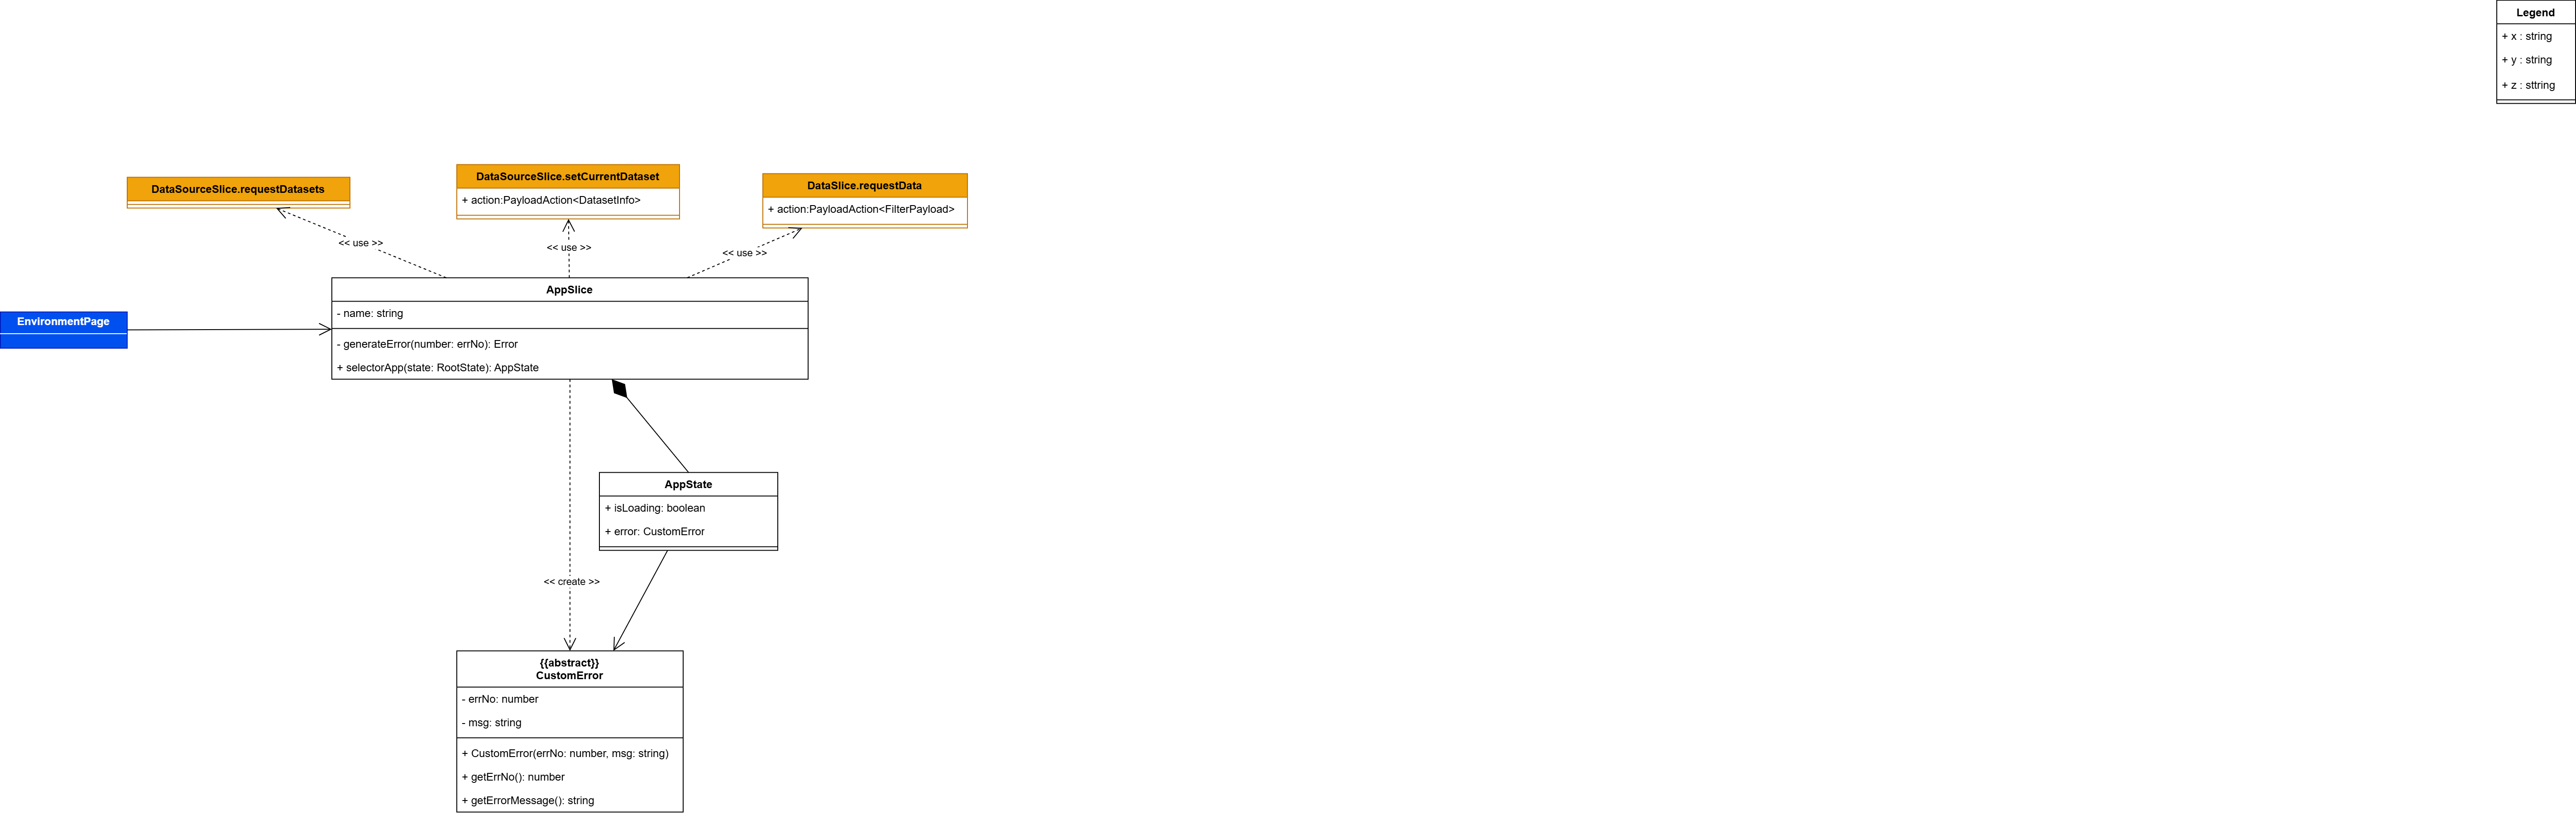
\includegraphics[scale=0.4]{template/images/uml_front/logic/AppSlice.png}
      \caption{AppSlice}
\end{figure}
\textbf{Descrizione del diagramma:}\\
Questo diagramma mostra i componenti per la gestione dello stato dell'applicazione.
\begin{itemize}
      \item \textbf{AppSlice:}
            \begin{itemize}
                  \item \textbf{Dipendenze:}
                        \begin{itemize}
                              \item AppState (composizione): gestisce la creazione e la distruzione dell'istanza di
                                    AppState, che non è condivisa con altri componenti;
                              \item CustomError (dipendenza semplice <<create>>): responsabile della creazione
                                    degli oggetti di errore personalizzati;
                              \item DataSourceSlice.requestDatasets (dipendenza semplice <<use>>): cattura
                                    un'istanza di DataSourceSlice.requestDatasets e il reducer aggiorna lo stato
                                    dell'applicazione;
                              \item DataSourceSlice.setCurrentDataset (dipendenza semplice <<use>>): cattura
                                    un'istanza di DataSourceSlice.setCurrentDataset e il reducer aggiorna lo stato
                                    dell'applicazione;
                              \item DataSlice.requestData (dipendenza semplice <<use>>): cattura un'istanza di
                                    DataSlice.requestData e il reducer aggiorna lo stato dell'applicazione.
                        \end{itemize}
                  \item \textbf{Interazioni:}
                        \begin{itemize}
                              \item AppState: viene modificato in base alle action catturate dal reducer della
                                    slice.
                        \end{itemize}
                  \item \textbf{Action catturate:}
                        \begin{itemize}
                              \item DataSourceSlice.requestDatasets;
                              \item DataSourceSlice.setCurrentDataset;
                              \item DataSlice.requestData.
                        \end{itemize}
            \end{itemize}

      \item \textbf{AppState:}
            \begin{itemize}
                  \item \textbf{Dipendenze:}
                        \begin{itemize}
                              \item CustomError (associazione): contiene l'oggetto che rappresenta l'errore.
                        \end{itemize}
            \end{itemize}

      \item \textbf{EnvironmentPage:}
            \begin{itemize}
                  \item \textbf{Dipendenze:}
                        \begin{itemize}
                              \item AppSlice (associazione): contiene implicitamente un'istanza di AppSlice.
                        \end{itemize}
                  \item \textbf{Interazioni:}
                        \begin{itemize}
                              \item AppSlice: viene utilizzato il metodo selectorApp per reperire lo stato
                                    dell'applicazione.
                        \end{itemize}
            \end{itemize}

      \item \textbf{HomePage:}
      \begin{itemize}
            \item \textbf{Dipendenze:}
                  \begin{itemize}
                        \item AppSlice (associazione): contiene implicitamente un'istanza di AppSlice.
                  \end{itemize}
            \item \textbf{Interazioni:}
                  \begin{itemize}
                        \item AppSlice: viene utilizzato il metodo selectorApp per reperire lo stato
                              dell'applicazione.
                  \end{itemize}
      \end{itemize}

      \item \textbf{ErrorPage:}
            \begin{itemize}
                  \item \textbf{Dipendenze:}
                        \begin{itemize}
                              \item AppSlice (associazione): contiene implicitamente un'istanza di AppSlice.
                        \end{itemize}
                  \item \textbf{Interazioni:}
                        \begin{itemize}
                              \item AppSlice: viene utilizzato il metodo selectorApp per reperire lo stato
                                    dell'applicazione.
                        \end{itemize}
            \end{itemize}
\end{itemize}

\subparagraph{CustomError}
\begin{center}
      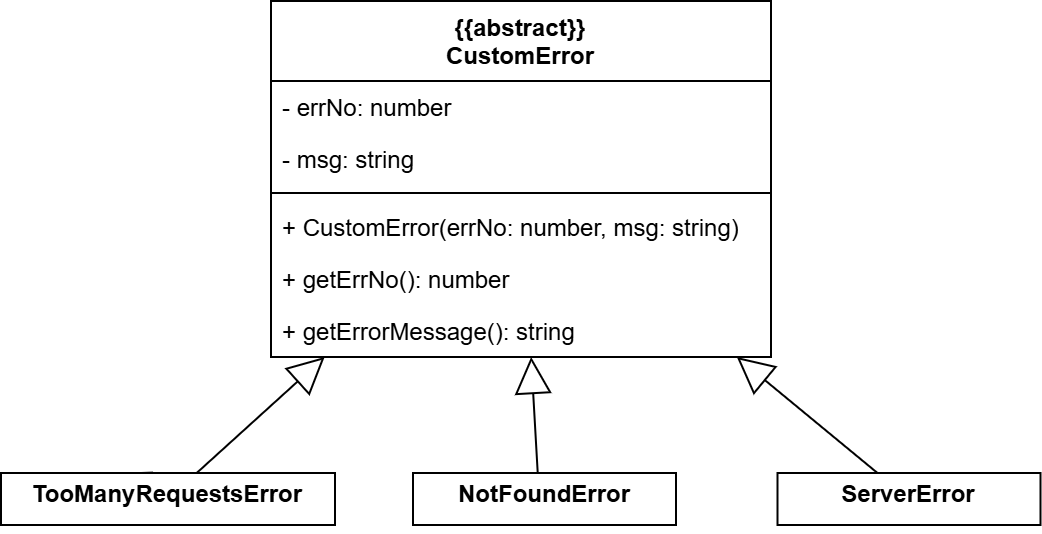
\includegraphics[scale=0.6]{template/images/uml_front/logic/CustomError.png}
      \captionof{figure}{CustomError}
\end{center}
\textbf{Descrizione del diagramma:}\\
Questo diagramma mostra tutte le classi di errore.
\begin{itemize}
      \item \textbf{TooManyRequestsError:}
            \begin{itemize}
                  \item \textbf{Dipendenze:}
                        \begin{itemize}
                              \item CustomError (generalizzazione): estende una classe CustomError personalizzata,
                                    derivata da una superclasse Error di TypeScript, che include un messaggio
                                    specifico per gli errori dovuti al superamento del limite di richieste.
                        \end{itemize}
            \end{itemize}

      \item \textbf{NotFoundError:}
            \begin{itemize}
                  \item \textbf{Dipendenze:}
                        \begin{itemize}
                              \item CustomError (generalizzazione): estende una classe CustomError personalizzata,
                                    derivata da una superclasse Error di TypeScript, che include un messaggio
                                    specifico per gli errori causati da un tentativo fallito di reperimento ai
                                    dati.
                        \end{itemize}
            \end{itemize}

      \item \textbf{ServerError:}
            \begin{itemize}
                  \item \textbf{Dipendenze:}
                        \begin{itemize}
                              \item CustomError (generalizzazione): estende una classe CustomError personalizzata,
                                    derivata da una superclasse Error di TypeScript, che include un messaggio
                                    specifico per gli errori interni al server.
                        \end{itemize}
            \end{itemize}
\end{itemize}

\pagebreak

\paragraph{FilterOptionSlice}
\begin{figure}[h!] \centering
      \includegraphics[scale=0.45]{template/images/uml_front/logic/FilterOptionSlice.png}
      \caption{FilterOptionSlice}
\end{figure}
\textbf{Descrizione del diagramma:}\\
Questo diagramma mostra i componenti per aggiornare e condividere le opzioni di filtraggio.
\begin{itemize}
      \item \textbf{FilterOptionSlice:}
            \begin{itemize}
                  \item \textbf{Dipendenze:}
                        \begin{itemize}
                              \item FilterOptionState (composizione): gestisce la creazione e la distruzione
                                    dell'istanza di FilterOptionState, che non è condivisa con altri componenti;
                              \item FilterOptionSlice.toggleIsGreater (dipendenza semplice <<use>>): cattura
                                    un'istanza di FilterOptionSlice.toggleIsGreater e il reducer imposta il tipo di
                                    filtraggio da effettuare utilizzando il payload.
                        \end{itemize}
                  \item \textbf{Interazioni:}
                        \begin{itemize}
                              \item FilterOptionState: viene modificato in base alle action catturate dal reducer
                                    della slice.
                        \end{itemize}
                  \item \textbf{Action catturate:}
                        \begin{itemize}
                              \item FilterOptionSlice.toggleIsGreater.
                        \end{itemize}
            \end{itemize}

      \item \textbf{Options:}
            \begin{itemize}
                  \item \textbf{Dipendenze:}
                        \begin{itemize}
                              \item FilterOptionSlice (associazione): contiene implicitamente un'istanza di
                                    FilterOptionSlice.
                        \end{itemize}
                  \item \textbf{Interazioni:}
                        \begin{itemize}
                              \item FilterOptionSlice: viene utilizzato il metodo selectorIsGreater per reperire le
                                    opzioni per il filtraggio.
                        \end{itemize}
            \end{itemize}

      \item \textbf{BarChart:}
            \begin{itemize}
                  \item \textbf{Dipendenze:}
                        \begin{itemize}
                              \item FilterOptionSlice (associazione): contiene implicitamente un'istanza di
                                    FilterOptionSlice.
                        \end{itemize}
                  \item \textbf{Interazioni:}
                        \begin{itemize}
                              \item FilterOptionSlice: viene utilizzato il metodo selectorIsGreater per reperire le
                                    opzioni per il filtraggio.
                        \end{itemize}
            \end{itemize}

      \item \textbf{DataTable:}
            \begin{itemize}
                  \item \textbf{Dipendenze:}
                        \begin{itemize}
                              \item FilterOptionSlice (associazione): contiene implicitamente un'istanza di
                                    FilterOptionSlice.
                        \end{itemize}
                  \item \textbf{Interazioni:}
                        \begin{itemize}
                              \item FilterOptionSlice: viene utilizzato il metodo selectorIsGreater per reperire le
                                    opzioni per il filtraggio.
                        \end{itemize}
            \end{itemize}

      \item \textbf{FilterModOption:}
            \begin{itemize}
                  \item \textbf{Dipendenze:}
                        \begin{itemize}
                              \item FilterOptionSlice.toggleIsGreater (associazione semplice <<send>>): crea ed
                                    emette un'istanza dell'action FilterOptions.toggleIsGreater.
                        \end{itemize}
                  \item \textbf{Action emesse:}
                        \begin{itemize}
                              \item FilterOptionSlice.toggleIsGreater.
                        \end{itemize}
            \end{itemize}
\end{itemize}

\paragraph{ViewOptionSlice}
\begin{figure}[h!] \centering
      \includegraphics[scale=0.45]{template/images/uml_front/logic/ViewOptionSlice.png}
      \caption{ViewOptionSlice}
\end{figure}
\textbf{Descrizione del diagramma:}\\
Questo diagramma mostra i componenti per aggiornare e condividere le opzioni di visibilità del piano medio.
\begin{itemize}
      \item \textbf{ViewOptionSlice:}
            \begin{itemize}
                  \item \textbf{Dipendenze:}
                        \begin{itemize}
                              \item ViewOptionState (composizione): gestisce la creazione e la distruzione
                                    dell'istanza di ViewOptionState, che non è condivisa con altri componenti;
                              \item ViewOptionSlice.toggleAveragePlane (dipendenza semplice <<use>>): cattura
                                    un'istanza di ViewOptionSlice.toggleAveragePlane e il reducer imposta la
                                    visibilità del piano medio utilizzando il payload;
                        \end{itemize}
                  \item \textbf{Interazioni:}
                        \begin{itemize}
                              \item ViewOptionState: viene modificato in base alle action catturate dal reducer
                                    della slice.
                        \end{itemize}
                  \item \textbf{Action catturate:}
                        \begin{itemize}
                              \item ViewOptionSlice.toggleAveragePlane;
                        \end{itemize}
            \end{itemize}

      \item \textbf{AveragePlaneOption:}
            \begin{itemize}
                  \item \textbf{Dipendenze:}
                        \begin{itemize}
                              \item ViewOptionSlice.toggleAveragePlane (associazione semplice <<send>>): crea ed
                                    emette un'istanza dell'action ViewOptionSlice.toggleAveragePlane.
                        \end{itemize}
                  \item \textbf{Action emesse:}
                        \begin{itemize}
                              \item ViewOptionSlice.toggleAveragePlane.
                        \end{itemize}
            \end{itemize}

      \item \textbf{AveragePlane:}
            \begin{itemize}
                  \item \textbf{Dipendenze:}
                        \begin{itemize}
                              \item ViewOptionSlice (associazione): contiene implicitamente un'istanza di
                                    ViewOptionSlice.
                        \end{itemize}
                  \item \textbf{Interazioni:}
                        \begin{itemize}
                              \item ViewOptionSlice: viene utilizzato il metodo selectorIsPlaneActive per reperire
                                    le opzioni di visibilità.
                        \end{itemize}
            \end{itemize}

\end{itemize}

\paragraph{RaycastHitSlice}
\begin{figure}[h!] \centering
      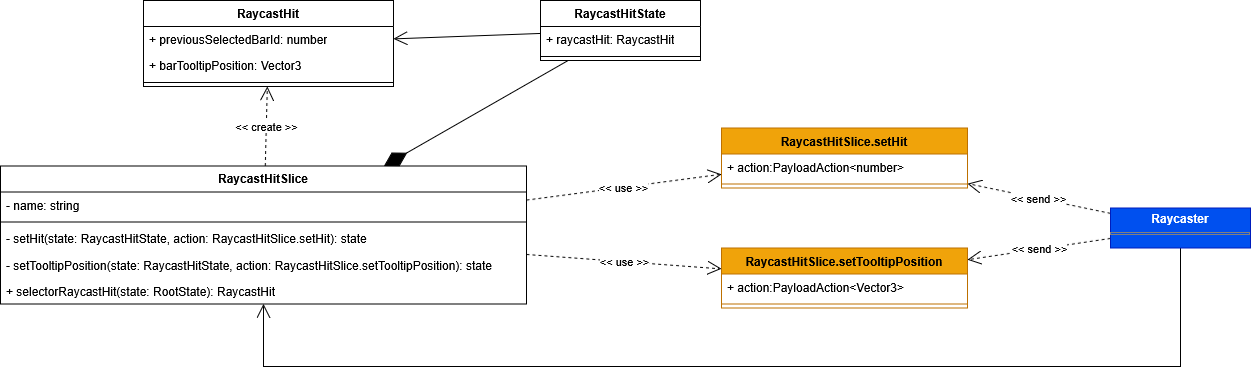
\includegraphics[scale=0.4]{template/images/uml_front/logic/raycastslice.png}
      \caption{RaycastHitSlice}
\end{figure}
\textbf{Descrizione del diagramma:}\\
Questo diagramma mostra i componenti per aggiornare e condividere le informazioni relative al raycasting.
\begin{itemize}
      \item \textbf{RaycastHitSlice:}
            \begin{itemize}
                  \item \textbf{Dipendenze:}
                        \begin{itemize}
                              \item RaycastHitState (composizione): gestisce la creazione e la distruzione
                                    dell'istanza di RaycastHitState, che non è condivisa con altri componenti;
                              \item RaycastHitSlice.setHit (dipendenza semplice <<use>>): cattura un'istanza di
                                    RaycastHitSlice.setHit e il reducer memorizza la barra del grafico cliccata
                                    dall'utente utilizzando il payload;
                              \item RaycastHitSlice.setTooltipPosition (dipendenza semplice <<use>>): cattura
                                    un'istanza di RaycastHitSlice.setTooltipPosition e il reducer aggiorna la
                                    posizione del tooltip utilizzando il payload.
                        \end{itemize}
                  \item \textbf{Interazioni:}
                        \begin{itemize}
                              \item RaycastHitState: viene modificato in base alle action catturate dal reducer
                                    della slice.
                        \end{itemize}
                  \item \textbf{Action catturate:}
                        \begin{itemize}
                              \item RaycastHitSlice.setHit;
                              \item RaycastHitSlice.setTooltipPosition.
                        \end{itemize}
            \end{itemize}

      \item \textbf{BarChart:}
            \begin{itemize}
                  \item \textbf{Dipendenze:}
                        \begin{itemize}
                              \item RaycastHitSlice (associazione): contiene implicitamente un'istanza di
                                    RaycastHitSlice;
                              \item RaycastHitSlice.setHit (dipendenza semplice <<send>>): crea ed emette
                                    un'istanza dell'action RaycastHitSlice.setHit;
                              \item RaycastHitSlice.setTooltipPosition (dipendenza semplice <<send>>): crea ed
                                    emette un'istanza dell'action RaycastHitSlice.setTooltipPosition.
                        \end{itemize}
                  \item \textbf{Interazioni:}
                        \begin{itemize}
                              \item RaycastHitSlice: viene utilizzato il metodo selectorRaycastHit per reperire le
                                    informazioni relative al raycasting.
                        \end{itemize}
                  \item \textbf{Action emesse:}
                        \begin{itemize}
                              \item RaycastHitSlice.setHit;
                              \item RaycastHitSlice.setTooltipPosition.
                        \end{itemize}
            \end{itemize}

      \item \textbf{Options:}
            \begin{itemize}
                  \item \textbf{Dipendenze:}
                        \begin{itemize}
                              \item RaycastHitSlice.setHit (associazione semplice <<send>>): crea ed
                                    emette un'istanza dell'action RaycastHitSlice.setHit.
                        \end{itemize}
                  \item \textbf{Action emesse:}
                        \begin{itemize}
                              \item RaycastHitSlice.setHit.
                        \end{itemize}
            \end{itemize}

      \item \textbf{DataTable:}
            \begin{itemize}
                  \item \textbf{Dipendenze:}
                        \begin{itemize}
                              \item RaycastHitSlice.setHit (associazione semplice <<send>>): crea ed
                                    emette un'istanza dell'action RaycastHitSlice.setHit.
                        \end{itemize}
                  \item \textbf{Action emesse:}
                        \begin{itemize}
                              \item RaycastHitSlice.setHit.
                        \end{itemize}
            \end{itemize}

      \item \textbf{Tooltip:}
            \begin{itemize}
                  \item \textbf{Dipendenze:}
                        \begin{itemize}
                              \item RaycastHitSlice (associazione): contiene implicitamente un'istanza di
                                    RaycastHitSlice;
                        \end{itemize}
                  \item \textbf{Interazioni:}
                        \begin{itemize}
                              \item RaycastHitSlice: viene utilizzato il metodo selectorRaycastHit per reperire le
                                    informazioni relative al raycasting.
                        \end{itemize}
            \end{itemize}

      \item \textbf{Bars:}
            \begin{itemize}
                  \item \textbf{Dipendenze:}
                        \begin{itemize}
                              \item RaycastHitSlice (associazione): contiene implicitamente un'istanza di
                                    RaycastHitSlice;
                        \end{itemize}
                  \item \textbf{Interazioni:}
                        \begin{itemize}
                              \item RaycastHitSlice: viene utilizzato il metodo selectorRaycastHit per reperire le
                                    informazioni relative al raycasting.
                        \end{itemize}
            \end{itemize}
\end{itemize}

\paragraph{Redux store}
\begin{figure}[h!] \centering
      \includegraphics[scale=0.35]{template/images/uml_front/logic/Store.png}
      \caption{Redux store}
\end{figure}
\textbf{Descrizione del diagramma:}\\
Questo diagramma mostra lo store e le slice che compongono lo stato globale dell'applicazione.
\begin{itemize}
      \item \textbf{Store:}
            \begin{itemize}
                  \item \textbf{Dipendenze:}
                        \begin{itemize}
                              \item RootReducer (associazione): possiede un attributo RootReducer che permette di
                                    combinare più slice con cui lo store interagisce per modificare lo stato
                                    globale dell'applicazione.
                        \end{itemize}
            \end{itemize}

      \item \textbf{RootReducer:}
            \begin{itemize}
                  \item \textbf{Dipendenze:}
                        \begin{itemize}
                              \item DataSlice (associazione): possiede un attributo DataSlice per offrire allo
                                    store l'accesso alla slice;
                              \item DataSourceSlice (associazione): possiede un attributo DataSourceSlice per
                                    offrire allo store l'accesso alla slice;
                              \item FilterOptionSlice (associazione): possiede un attributo FilterOptionSlice per
                                    offrire allo store l'accesso alla slice;
                              \item ViewOptionSlice (associazione): possiede un attributo ViewOptionSlice per
                                    offrire allo store l'accesso alla slice;
                              \item AppSlice (associazione): possiede un attributo AppSlice per offrire allo store
                                    l'accesso alla slice;
                              \item RaycastHitSlice (associazione): possiede un attributo RaycastHitSlice per
                                    offrire allo store l'accesso alla slice.
                        \end{itemize}
            \end{itemize}
\end{itemize}

\pagebreak

\paragraph{Pages}
\begin{figure}[h!] \centering
      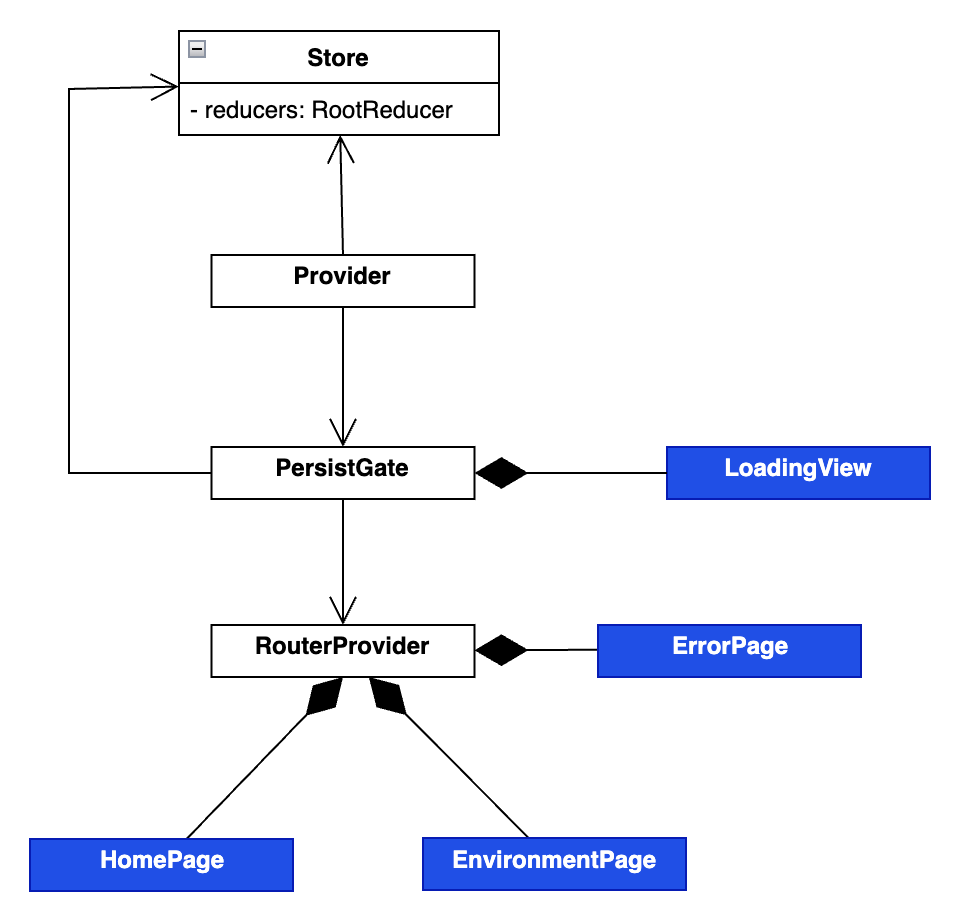
\includegraphics[scale=0.6]{template/images/uml_front/ui/pages.png}
      \caption{Pages}
\end{figure}
\textbf{Descrizione del diagramma:}
Questo diagramma mostra come sono organizzate le varie pagine dell'applicazione.
\begin{itemize}
      \item \textbf{Provider:}
            \begin{itemize}
                  \item \textbf{Dipendenze:}
                        \begin{itemize}
                              \item Store (associazione): utile al Provider di Redux per consentire l'accesso allo
                                    store (e quindi allo stato globale) a tutti i componenti nella gerarchia;
                              \item PersistGate (associazione): componente React che gestisce il caricamento
                                    dell'applicazione e il ripristino dello stato persistente;
                        \end{itemize}
            \end{itemize}

      \item \textbf{PersistGate:}
      \begin{itemize}
            \item \textbf{Dipendenze:}
                  \begin{itemize}
                        \item Store (associazione): utile per consentire l'accesso allo
                              store (e quindi allo stato globale);
                        \item LoadingView (composizione): componente React dedicato alla visualizzazione di un indi-
                              catore di caricamento;
                        \item RouterProvider (associazione): componente React che gestisce le pagine
                        dell'applicazione e le loro relative rotte.
                  \end{itemize}
      \end{itemize}

      \item \textbf{RouterProvider:}
            \begin{itemize}
                  \item \textbf{Dipendenze:}
                        \begin{itemize}
                              \item HomePage (composizione): componente React che rappresenta la pagina iniziale
                                    dell'applicazione;
                              \item EnvironmentPage (composizione): componente React che fornisce l'interfaccia per
                                    visualizzare un dataset in un ambiente 3D;
                              \item ErrorPage (composizione): componente React responsabile della visualizzazione e
                                    della gestione degli errori generati dall'applicazione.
                        \end{itemize}
            \end{itemize}
\end{itemize}

\pagebreak

\paragraph{HomePage}
\begin{figure}[h!] \centering
      \includegraphics[scale=0.3]{template/images/uml_front/ui/HomePage.png}
      \caption{HomePage}
\end{figure}
\textbf{Descrizione del diagramma:}
Questo diagramma presenta l'organizzazione degli elementi all'interno della pagina iniziale dell'applicazione.
\begin{itemize}
      \item \textbf{HomePage:}
            \begin{itemize}
                  \item \textbf{Dipendenze:}
                        \begin{itemize}
                              \item APISelector (composizione): componente React che offre all'utente l'interfaccia
                                    per la scelta del dataset desiderato;
                              \item Footer (composizione): componente React dedicato alla visualizzazione del
                                    footer dell'applicazione;
                        \end{itemize}
            \end{itemize}

      \item \textbf{APISelector:}
            \begin{itemize}
                  \item \textbf{Dipendenze:}
                        \begin{itemize}
                              \item DatasetItem (composizione): componente React dedicato alla presentazione delle
                                    informazioni relative a un dataset
                        \end{itemize}
            \end{itemize}
\end{itemize}

\paragraph{EnvironmentPage}
\begin{figure}[h!] \centering
      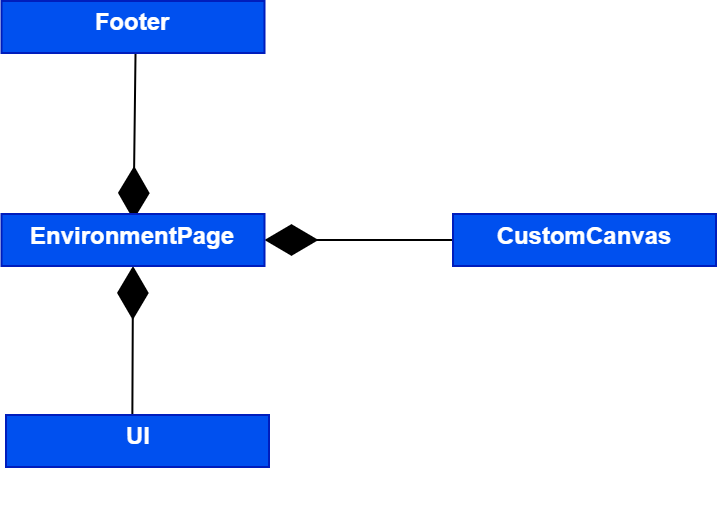
\includegraphics[scale=0.6]{template/images/uml_front/ui/EnvironmentPage.png}
      \caption{EnvironmentPage}
\end{figure}
\textbf{Descrizione del diagramma:}
Questo diagramma presenta l'organizzazione degli elementi all'interno della pagina dedicata alla visualizzazione di un dataset in ambiente 3D.
\begin{itemize}
      \item \textbf{EnvironmentPage:}
            \begin{itemize}
                  \item \textbf{Dipendenze:}
                        \begin{itemize}
                              \item UI (composizione): componente React che avvolge e gestisce l'intera UI
                                    dell'applicazione;
                              \item CustomCanvas (composizione): componente React responsabile della
                                    visualizzazione e del rendering dell'ambiente 3D;
                              \item LoadingView (composizione): componente React dedicato alla visualizzazione di un indicatore di
                                    caricamento;
                        \end{itemize}
            \end{itemize}
\end{itemize}

\paragraph{UI}
\begin{figure}[h!] \centering
      \includegraphics[scale=0.3]{template/images/uml_front/ui/UI.png}
      \caption{UI}
\end{figure}
\textbf{Descrizione del diagramma:}
Questo diagramma presenta la struttura e gli elementi che costituiscono la UI dell'applicazione.
\begin{itemize}
      \item \textbf{UI:}
            \begin{itemize}
                  \item \textbf{Dipendenze:}
                        \begin{itemize}
                              \item DataTable (composizione): componente React dedicato alla presentazione di un
                                    dataset in formato tabellare;
                              \item Options (composizione): componente React dedicato alla visualizzazione di un
                                    form contenente le opzioni di filtraggio e visibilità del piano medio.
                        \end{itemize}
            \end{itemize}

      \item \textbf{DataTable:}
            \begin{itemize}
                  \item \textbf{Dipendenze:}
                        \begin{itemize}
                              \item ExpandedButton (composizione): componente React che implementa un pulsante per
                                    espandere o comprimere la tabella e le opzioni.
                        \end{itemize}
            \end{itemize}
\end{itemize}

\paragraph{Options}
\begin{figure}[h!] \centering
      \includegraphics[scale=0.3]{template/images/uml_front/ui/Options.png}
      \caption{Options}
\end{figure}
\textbf{Descrizione del diagramma:}
Questo diagramma evidenzia la struttura dei gruppi in cui sono suddivise le opzioni di filtraggio e visibilità del piano medio.
\begin{itemize}
      \item \textbf{Options:}
            \begin{itemize}
                  \item \textbf{Dipendenze:}
                        \begin{itemize}
                              \item NFilter (composizione): componente React che offre la possibilità eseguire un
                                    filtraggio sul dataset visualizzando solo i primi N valori più alti o più
                                    bassi;
                              \item Filter (composizione): componente React che implementa un filtro generico
                                    capace di eseguire un filtraggio visualizzando valori superiori o inferiori
                                    rispetto a un dato valore di riferimento;
                              \item FilterModOption (composizione): componente React che visualizza un form per
                                    permettere all'utente di scegliere se il filtro opererà su valori maggiori o
                                    minori;
                              \item AveragePlaneOption (composizione): componente React che implementa un filtro
                                    generico capace di filtrare valori superiori o inferiori rispetto a un dato
                                    valore di riferimento;
                              \item ExpandedButton (composizione): componente React che implementa un pulsante per
                                    espandere o comprimere la tabella e le opzioni;
                        \end{itemize}
            \end{itemize}
      \item \textbf{NFilter:}
            \begin{itemize}
                  \item \textbf{Dipendenze:}
                        \begin{itemize}
                              \item Filter (associazione): componente React che implementa un filtro generico
                                    capace di filtrare valori superiori o inferiori rispetto a un dato valore di
                                    riferimento. In questo caso, è stato esteso per includere un campo che permette
                                    di specificare un valore N.
                        \end{itemize}
            \end{itemize}
\end{itemize}


\paragraph{CustomCanvas}
\begin{figure}[h!] \centering
      \includegraphics[scale=0.3]{template/images/uml_front/ui/CustomCanvas.png}
      \caption{CustomCanvas}
\end{figure}
\textbf{Descrizione del diagramma:}
Questo diagramma presenta la struttura e gli elementi che costituiscono l'ambiente 3D.
\begin{itemize}
      \item \textbf{CustomCanvas:}
            \begin{itemize}
                  \item \textbf{Dipendenze:}
                        \begin{itemize}
                              \item OrbitControls (composizione): componente React Three Drei che abilita la
                                    navigazione e la manipolazione della telecamera 3D utilizzando gli input del
                                    mouse;
                              \item BarChart (composizione): componente React che racchiude e gestisce l'intera
                                    struttura del grafico 3D.
                        \end{itemize}
            \end{itemize}
\end{itemize}

\paragraph{BarChart}
\begin{figure}[h!] \centering
      \includegraphics[scale=0.3]{template/images/uml_front/ui/BarChart.png}
      \caption{BarChart}
\end{figure}
\textbf{Descrizione del diagramma:}
Questo diagramma presenta gli elementi che costituiscono il grafico 3D.
\begin{itemize}
      \item \textbf{BarChart:}
            \begin{itemize}
                  \item \textbf{Dipendenze:}
                        \begin{itemize}
                              \item Axes (composizione): componente React che contiene gli assi X, Y e Z del
                                    grafico 3D;
                              \item AveragePlane (composizione): componente React che permette di visualizzare il
                                    piano medio sul grafico 3D;
                              \item Lights (composizione): componente React per la gestione delle luci
                                    nell'ambiente 3D;
                              \item Tooltip (composizione): componente React per visualizzare un riquadro
                                    informativo al passaggio del mouse sopra la barra del grafico;
                              \item Bars (composizione): componente React dedicato al rendering degli elementi che
                                    rappresentano le barre all'interno del grafico 3D.
                        \end{itemize}
            \end{itemize}
      \item \textbf{Lights:}
            \begin{itemize}
                  \item \textbf{Dipendenze:}
                        \begin{itemize}
                              \item AmbientLight (composizione): componente React Three Fiber che fornisce
                                    un'illuminazione uniforme senza ombre alla scena 3D;
                              \item PointLight (composizione): componente React Three Fiber che fornisce
                                    un'illuminazione emessa da un punto verso tutte le direzioni nella scena 3D.
                        \end{itemize}
            \end{itemize}
\end{itemize}

\paragraph{Axes}
\begin{figure}[h!] \centering
      \includegraphics[scale=0.3]{template/images/uml_front/ui/Axes.png}
      \caption{Axes}
\end{figure}
\textbf{Descrizione del diagramma:}
Questo diagramma presenta gli elementi che costituiscono ciascuno dei tre assi del grafico 3D.
\begin{itemize}
      \item \textbf{Axes:}
            \begin{itemize}
                  \item \textbf{Dipendenze:}
                        \begin{itemize}
                              \item Axis (composizione): componente React che rappresenta un generico asse del
                                    grafico 3D con relative etichette.
                        \end{itemize}
            \end{itemize}
\end{itemize}